\section{Context Survey}
\renewcommand{\imgpath}{tex/litreview/imgs}

\subsection{Previous work}
The dataset of lobster images used in this project are taken from the master's thesis of Abdallah A. Abdallah \cite{lobster-thesis}. In his work, Abdallah created the dataset consisting of images and features of lobsters with help and advice from the Scottish Oceans Institute. The lobsters were measured and categorised and segmentation and feature extraction techniques were applied to create a more diverse dataset with baseline results. Additionally, machine learning techniques of classification and regression were used to classify the category (juvenile or mature) and sex of the lobsters and to predict the carapace length. 
\n
The methods used in Abdallah's work were simple in that to be able to segment the lobsters from the image backgrounds, a high contrasting background was required, meaning the method was prone to noise. Further, his method of feature extraction using linear regression and principle component analysis was based mostly on the shapes of the segmented images, which were negatively affected by the posture of the lobster and asymmetric lobster shapes. This project uses a new, more complex approach with feature detectors and graph matching for a more accurate evaluation by automatically detecting the individual parts of a lobster to overcome issues of noise and shape. 

\subsection{Related work}

\subsubsection{Human pose recognition}
The use of graphs in human pose estimation has been studied in the past
\cite{human-pose, human-skeleton} where labelled nodes that represent important features such as hands and heads are used to build skeleton models.
\n
Some of the methodology used in human pose estimation can be applied to our lobster matching problem. In particular, the paper on human pose estimation using a topological graph database by Tanaka et al. \cite{human-pose} uses a graph matching technique with an attributed graph to match skeletons to corresponding human postures. In their paper, example skeletons with different human topologies are developed into attributed graphs with manually assigned body part labels and stored in a model graph database. Any input skeletons can then also be converted to an attributed graph and matched with the examples in the database. Because their method of subgraph matching produces multiple results, further filters were needed to reduce the remaining graphs to one correct match. 
\imagefig{0.6\textwidth}{\imgpath/human-pose.png}{Body part identification algorithm using a model graph database (MGDB). Reproduced from \cite{human-pose}.}
\noindent
The aspect of having labelled attributed graphs of human skeletons extends well to labelled graphs of lobsters. In the methodology of this project - which is explained in section \ref{sec:design} - some parts of Tanaka's method were followed. Most notably, the use of example lobster graphs stored in a database for input subgraphs to match to as an initial filter and the application of further techniques from the matched results to arrive at the final lobster graph were all inspired by Tanaka's paper.
 
\subsubsection{Cattle identification} \label{sec:cattle}
The concept of combining local invariant features (keypoints) and graph matching has also been studied for use in automatic cattle identification \cite{cattle}. The application of feature extraction and graph matching in Monteiro's paper is different from the approach taken in this project, but it showed the concept of combining feature extraction with computer vision algorithms and graph matching could be used in complement as the graph structure is able to preserve the point neighbouring structure of extracted features. This is relevant to the problem of lobster part identification as different body parts have a clear neighbouring structure with other body parts.
\n
In the paper, the goal of graph matching was to match images of the same muzzle as a means of identification (like human fingerprints). This is similar to classic computer vision matching with k-nearest neighbours matching between keypoints to match objects in a scene. The paper shows how graph matching with attributed graphs can take advantage of the associated attributes in each node and edge to represent the relationship between two features. Aspects of this are used in the final stages of graph creation (section \ref{sec:graph-creation}) when building the full lobster graph from a pool of smaller labelled subgraphs. 

\subsection{Graph matching problem}
The graph matching, or subgraph isomorphism problem is where, given two undirected graphs $G_1$ and $G_2$, it must be determined whether the graph $G_1$ contains a subgraph that is isomorphic to $G_2$ \cite{subgraph}. Cook showed in his paper that subgraph isomorphism was NP-complete with a reduction to the 3-SAT problem. This problem applies to the project from the use of subgraph matching to determine if a labelled subgraph is contained in a larger complete graph of a lobster. 
\begin{figure}[H]
\centering
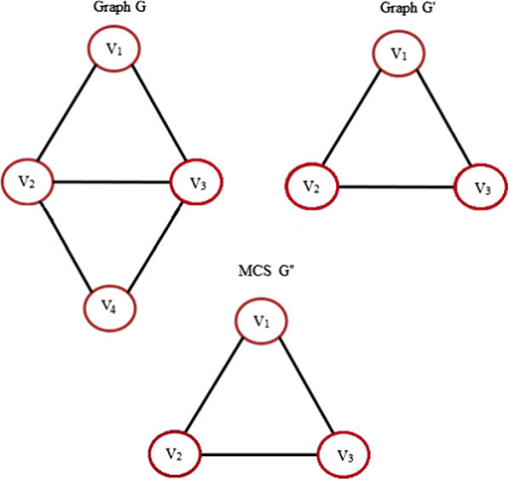
\includegraphics[width=0.5\textwidth]{\imgpath/graph-matching.png}
\caption{Example of matching two graphs $G$ and $G'$ and the resultant Maximum Common Subgraph ($MCS$). The MCS is simply a subgraph of both $G$ and $G'$ which contains the maximum number of nodes of all possible subgraphs of $G$ and $G'$ \cite{graph-matching}.}
\end{figure}
\noindent
In this project, the problem of graph matching extends beyond that of pure subgraph isomorphism, where only the number of vertices and its connections are relevant, though the normal subgraph isomorphism problem is also applied as part of the method pipeline. The extension comes from the fact that the shape of the lobster is a crucial part in determining successful matches. As was mentioned  in section \ref{sec:cattle}, the size of each node in the graph and the length (weight) of the edges are all important aspects in matching and are included during the final matching step. This leads to two different graph matching steps used in methodology of this project. First, the normal subgraph isomorphism problem is applied to get a list of matched subgraphs, then another complicated problem of rebuilding the complete graph from a list of subgraphs is solved to get to the final lobster graph, where the size of nodes and lengths of edges play a larger role.
